%=======================================================================
%  Satellite embeddings, text and night lights for municipal GDP -- mid-term review
%  Design: night-lights slides open and close the talk; content slides are map paper.
%  One colour per ingredient, everywhere (maps, charts, diagrams):
%     embeddings = teal   text = violet   night lights = amber   official GDP = brick   POI/roads = blue
%  The footer is a route line through the talk: Problem, Approach, Data, Test, Results, Next.
%  Build on the server (XeLaTeX, Lato):
%     python presentation/midterm/make_figures.py
%     cd presentation/midterm && latexmk -xelatex slides.tex
%=======================================================================
\documentclass[aspectratio=169,10pt]{beamer}
\usefonttheme{professionalfonts}
\usepackage{fontspec}
\setsansfont{Lato}
\newfontfamily\blackfont{Lato Black}
\newfontfamily\lightfont{Lato Light}
\usepackage{amsmath,amssymb}
\usepackage{booktabs,array,graphicx,xcolor}
\usepackage[normalem]{ulem}
\usepackage{tikz}
\usetikzlibrary{arrows.meta,positioning,calc,fit,backgrounds}
\graphicspath{{assets/}}

%------------------------- palette (same hex as make_figures.py) --------
\definecolor{night}{HTML}{0B1328}
\definecolor{night2}{HTML}{16223F}
\definecolor{glow}{HTML}{F2B134}
\definecolor{paper}{HTML}{F7F5F0}
\definecolor{ink}{HTML}{1E2433}
\definecolor{muted}{HTML}{687082}
\definecolor{rule}{HTML}{D9D5CC}
\definecolor{cimg}{HTML}{138A8A}
\definecolor{ctxt}{HTML}{7057C9}
\definecolor{cntl}{HTML}{E19A1F}
\definecolor{cgdp}{HTML}{C4493B}
\definecolor{cpoi}{HTML}{4A6FA5}
\definecolor{okc}{HTML}{2E8B57}
\definecolor{haze}{HTML}{AEB8D0}

%------------------------- beamer basics --------------------------------
\setbeamertemplate{navigation symbols}{}
\setbeamersize{text margin left=0.6cm,text margin right=0.6cm}
\setbeamercolor{normal text}{fg=ink}
\setbeamercolor{structure}{fg=ink}
\setbeamercolor{alerted text}{fg=cgdp}
\setbeamerfont{frametitle}{size=\fontsize{15}{18},series=\bfseries}
\setbeamertemplate{itemize item}{\raisebox{0.25ex}{\color{muted}\rule{0.4em}{0.4em}}}
\setbeamertemplate{enumerate item}{\color{cntl}\bfseries\insertenumlabel}
\setbeamertemplate{footline}{\vskip0.78cm}   % room for the footer drawn in the background
\setbeamertemplate{frametitle}{%
  \vskip0.36cm%
  \begin{beamercolorbox}[wd=\paperwidth,leftskip=0.6cm,rightskip=0.6cm]{frametitle}%
    \usebeamerfont{frametitle}\color{ink}\insertframetitle\par\vskip4pt%
    {\color{glow}\rule{1.1cm}{2.2pt}}%
  \end{beamercolorbox}\vskip0.02cm}
\hyphenpenalty=10000 \exhyphenpenalty=10000

%------------------------- route line in the footer ---------------------
\gdef\curstage{0}
\newcommand{\setstage}[1]{\gdef\curstage{#1}}
\newcommand{\paperbg}{%
  
\begin{tikzpicture}
    \useasboundingbox (0,0) rectangle (\paperwidth,\paperheight);
    \fill[paper] (0,0) rectangle (\paperwidth,\paperheight);
    \draw[rule,line width=0.4pt] (0.6cm,0.62cm) -- (\paperwidth-0.6cm,0.62cm);
    \node[anchor=west,font=\fontsize{6.5}{8}\selectfont,text=muted,inner sep=0] at (0.6cm,0.36cm)
      {Hemant \ $\cdot$ \ GIS term project \ $\cdot$ \ mid-term review};
    \node[anchor=east,font=\bfseries\fontsize{7}{8}\selectfont,text=ink,inner sep=0] at (\paperwidth-0.6cm,0.36cm)
      {\insertframenumber\,/\,\inserttotalframenumber};
    \ifnum\curstage>0
      \draw[rule,line width=1.2pt] (\paperwidth-7.9cm,0.36cm) -- (\paperwidth-1.7cm,0.36cm);
      \ifnum\curstage>1 \draw[ink,line width=1.2pt] (\paperwidth-7.9cm,0.36cm) -- ++({(\curstage-1)*1.24cm},0); \fi
      \foreach \s [count=\i] in {Problem,Approach,Data,Test,Results,Next} {
        \coordinate (st) at ({\paperwidth-7.9cm+(\i-1)*1.24cm},0.36cm);
        \ifnum\i<\curstage
          \fill[ink] (st) circle (1.6pt);
          \node[anchor=south,font=\fontsize{5.5}{6}\selectfont,text=ink,inner sep=1.5pt] at (st) {\s};
        \else\ifnum\i=\curstage
          \fill[glow] (st) circle (3pt); \fill[ink] (st) circle (1.1pt);
          \node[anchor=south,font=\bfseries\fontsize{5.5}{6}\selectfont,text=ink,inner sep=3pt] at (st) {\s};
        \else
          \filldraw[fill=paper,draw=muted!60,line width=0.6pt] (st) circle (1.6pt);
          \node[anchor=south,font=\fontsize{5.5}{6}\selectfont,text=muted!80,inner sep=1.5pt] at (st) {\s};
        \fi\fi
      }
    \else\ifnum\curstage<0
      \node[anchor=east,font=\bfseries\fontsize{6.5}{8}\selectfont,text=muted,inner sep=0] at (\paperwidth-1.7cm,0.36cm) {BACKUP};
    \fi\fi
  \end{tikzpicture}}
\setbeamertemplate{background}{\paperbg}
\newcommand{\nightbg}{%
  
\begin{tikzpicture}
    \useasboundingbox (0,0) rectangle (\paperwidth,\paperheight);
    \shade[inner color=night2,outer color=night] (0,0) rectangle (\paperwidth,\paperheight);
  \end{tikzpicture}}

%------------------------- helpers --------------------------------------
\newcommand{\muted}[1]{{\color{muted}#1}}
\newcommand{\dotc}[1]{\tikz[baseline=-0.6ex]\fill[#1] (0,0) circle (2.3pt);}
\newcommand{\ing}[2]{\dotc{#1}\,{\bfseries\color{#1}#2}}   % ingredient name in its colour
\newcommand{\chip}[2]{{\setlength{\fboxsep}{1.8pt}\colorbox{#1}{\fontsize{6}{7}\selectfont\bfseries\color{white}\strut #2}}}
\newcommand{\kpi}[3]{{\blackfont\fontsize{20}{22}\selectfont\color{#1}#2}\\[0pt]{\fontsize{7.5}{9}\selectfont\color{muted}#3}}
\newcommand{\eyebrow}[2][muted]{{\fontsize{6.5}{8}\selectfont\bfseries\color{#1}\addfontfeatures{LetterSpace=8}\MakeUppercase{#2}}}
\newcommand{\fnote}[1]{{\fontsize{7}{8.5}\selectfont\color{muted}#1}}
% caption sentences (assets/caption_example.tex)
\newcommand{\keep}[1]{\item[{\color{okc}\checkmark}] #1}
\newcommand{\dropped}[2]{\item[{\color{cgdp}$\times$}] {\color{muted}\sout{#1}}\ {\fontsize{6}{7}\selectfont\bfseries\color{cgdp}#2}}
% framed image with a coloured edge
\newcommand{\framed}[3]{{\setlength{\fboxsep}{0pt}\setlength{\fboxrule}{1.2pt}\fcolorbox{#1}{white}{\includegraphics[#2]{#3}}}}
\newcommand{\btile}[3]{\begin{minipage}[t]{0.235\linewidth}\raggedright\framed{ctxt}{width=\linewidth}{#1}\\[4pt]
  \eyebrow[ctxt]{#2}\\[1pt]{\fontsize{7}{8.5}\selectfont #3}\end{minipage}}
% pipeline styles (parameterised styles must live outside frames)
\tikzset{stage/.style={draw=#1,line width=1.1pt,fill=white,text width=3.25cm,minimum height=1.6cm,align=center,
           inner sep=5pt,font=\footnotesize},
         feed/.style={-{Stealth[length=2.2mm]},line width=1pt,draw=#1}}
\newcolumntype{L}[1]{>{\raggedright\arraybackslash}p{#1}}
\setlength{\leftmargini}{1.1em}

\newcommand{\nMunis}{853}
\newcommand{\nCells}{575k}
\newcommand{\nCaptions}{10,000}
\newcommand{\nKept}{84\%}
\newcommand{\nHybridR}{0.52}
\newcommand{\nNtlR}{0.27}
\newcommand{\nBuildings}{10M}
\newcommand{\nHybridRMSE}{0.41}
\newcommand{\nNtlRMSE}{0.51}
\newcommand{\nSentences}{60,023}
\newcommand{\nDropFiller}{4,183}
\newcommand{\nDropBuilding}{1,108}
\newcommand{\nDropRoad}{1,039}
\newcommand{\nDropWater}{1,046}
\newcommand{\nDropIndustry}{1,130}
\newcommand{\nDropFarm}{732}
\newcommand{\nDropUrban}{66}
\newcommand{\nDropKeptN}{50,684}
\newcommand{\nCalibGain}{$-$21\%}
\newcommand{\nClipDropped}{246}
\newcommand{\RQone}{no clear effect ($\Delta$RMSE +0.007, 95\% CI [-0.028, +0.041])}
\newcommand{\RQfour}{V10 better ($\Delta$RMSE -0.028, 95\% CI [-0.050, -0.008])}

\newcommand{\bcapnameA}{Forest}\newcommand{\bcapA}{A predominantly forested area with patches of cleared land.}
\newcommand{\bcapnameB}{Farmland}\newcommand{\bcapB}{A large, circular area of brown farmland, likely recently plowed, dominating the center.}
\newcommand{\bcapnameC}{Village edge}\newcommand{\bcapC}{A sparsely built area with scattered houses and small buildings, likely residential.}
\newcommand{\bcapnameD}{Town centre}\newcommand{\bcapD}{A densely built-up area with numerous houses featuring red-tiled roofs, indicating a residential neighborhood.}


\begin{document}

%======================== 1. TITLE (night) =============================
{\setbeamertemplate{background}{\nightbg}
\begin{frame}[plain]
\begin{tikzpicture}[remember picture,overlay]
  \node[anchor=east,inner sep=0] (map) at ($(current page.east)+(1.0,0.1)$)
    {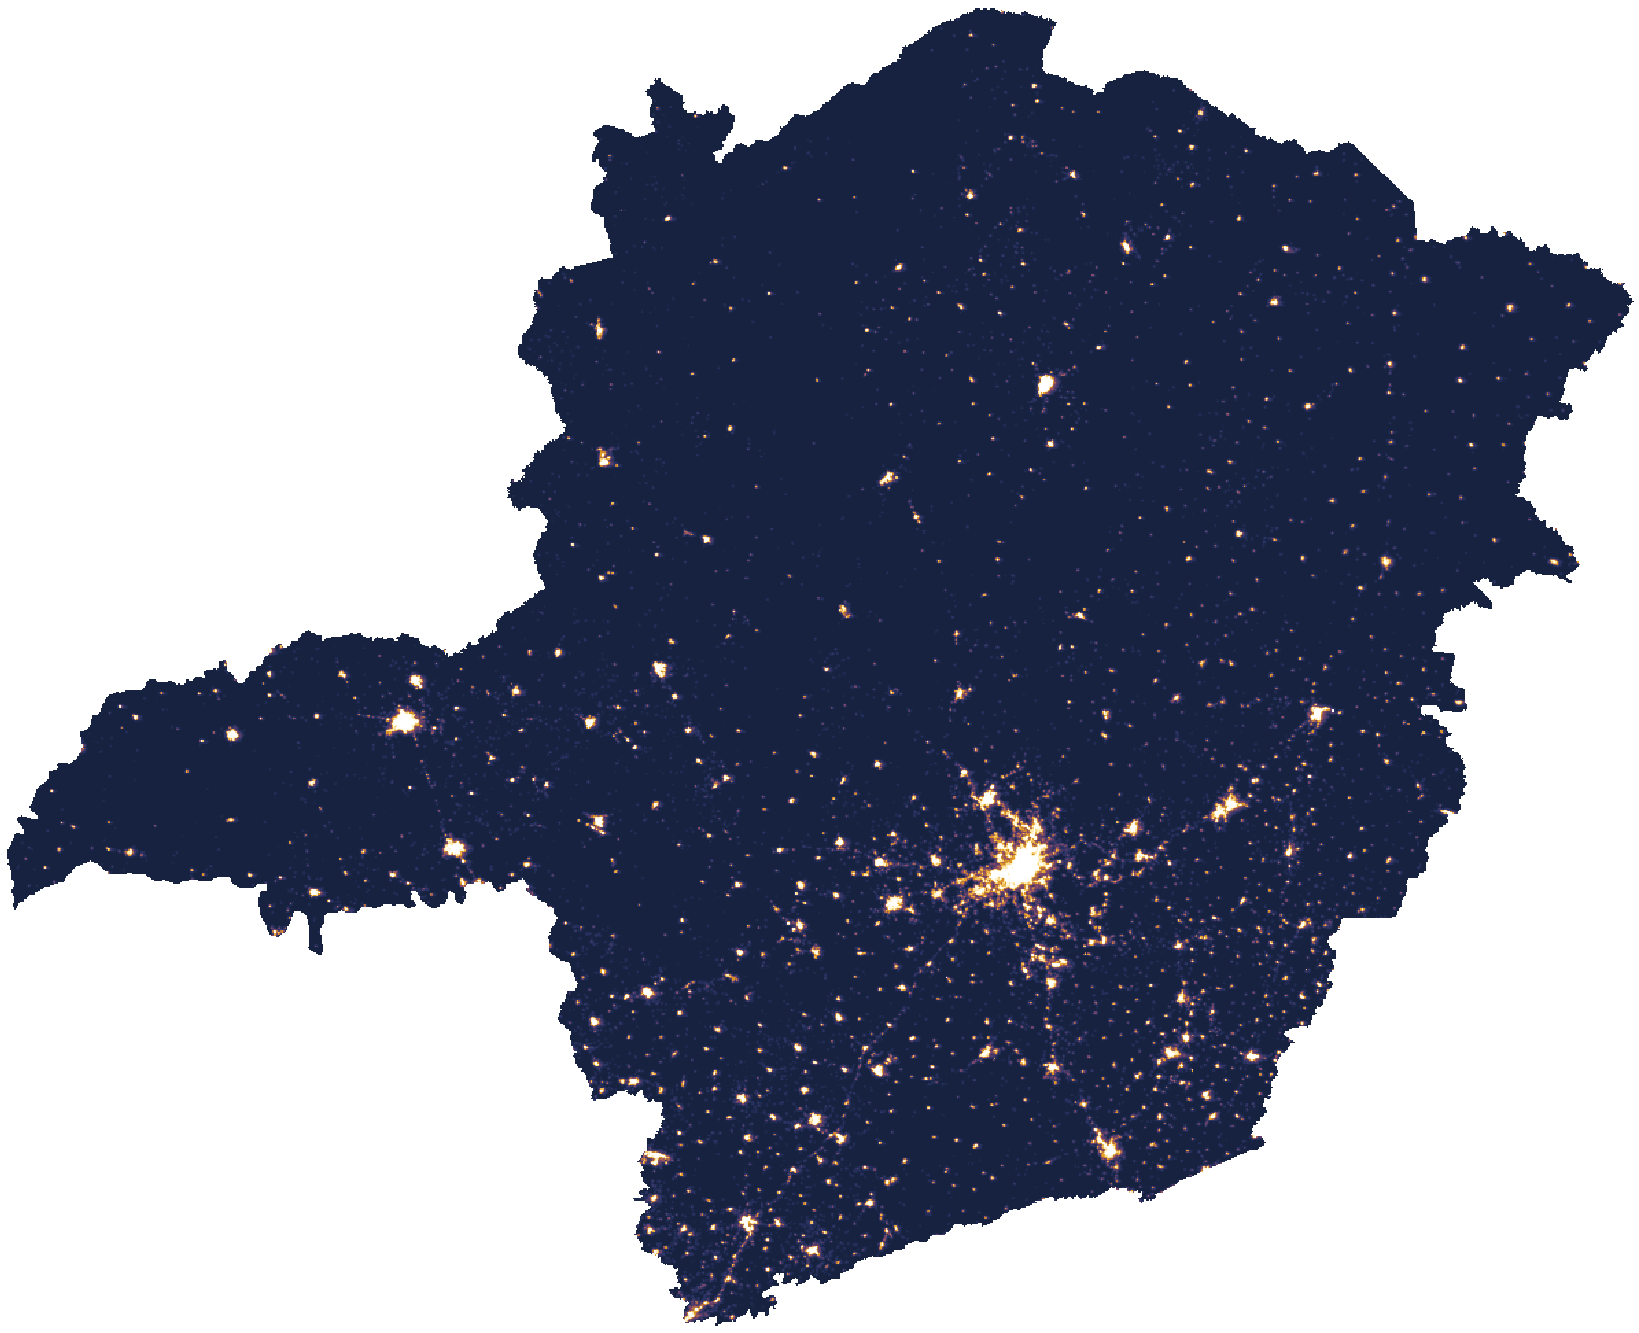
\includegraphics[height=0.96\paperheight]{hero_ntl.png}};
  \begin{scope}[x={($(map.south east)-(map.south west)$)},y={($(map.north west)-(map.south west)$)},shift={(map.south west)}]
    \draw[haze,line width=0.4pt] (0.625,0.345) -- (0.70,0.20) node[anchor=north west,inner sep=1pt,
      font=\fontsize{6.5}{8}\selectfont,text=haze] {Belo Horizonte};
    \draw[haze,line width=0.4pt] (0.245,0.465) -- (0.20,0.33) node[anchor=north,inner sep=1pt,
      font=\fontsize{6.5}{8}\selectfont,text=haze] {Uberlândia};
  \end{scope}
  \node[anchor=south east,font=\fontsize{6}{7}\selectfont,text=haze,align=right] at ($(current page.south east)+(-0.4,0.3)$)
    {VIIRS night lights 2022, one pixel per 1\,km cell};
\end{tikzpicture}
\begin{minipage}{0.47\textwidth}\raggedright
  \eyebrow[glow]{GIS term project \ $\cdot$ \ mid-term review}\\[10pt]
  {\blackfont\fontsize{24}{27}\selectfont\color{white}Reading the economy from space\par}
  \vspace{8pt}
  {\lightfont\fontsize{12}{15}\selectfont\color{white}Estimating municipal GDP from satellite embeddings, text and night lights\par}
  \vspace{12pt}
  {\color{glow}\rule{1.6cm}{2.2pt}}\\[10pt]
  {\fontsize{10}{12}\selectfont\bfseries\color{white}Hemant}\ {\fontsize{9}{11}\selectfont\color{haze}(22CS30029)}\\[4pt]
  {\fontsize{8}{10}\selectfont\color{haze}Minas Gerais, Brazil \ $\cdot$ \ \nMunis{} municipalities\\October 2026}
\end{minipage}
\end{frame}}

%======================== 2. PROBLEM ===================================
\setstage{1}
\begin{frame}{Local GDP is patchy; satellites see every place}
\begin{columns}[T,onlytextwidth]
\column{0.5\textwidth}
\centering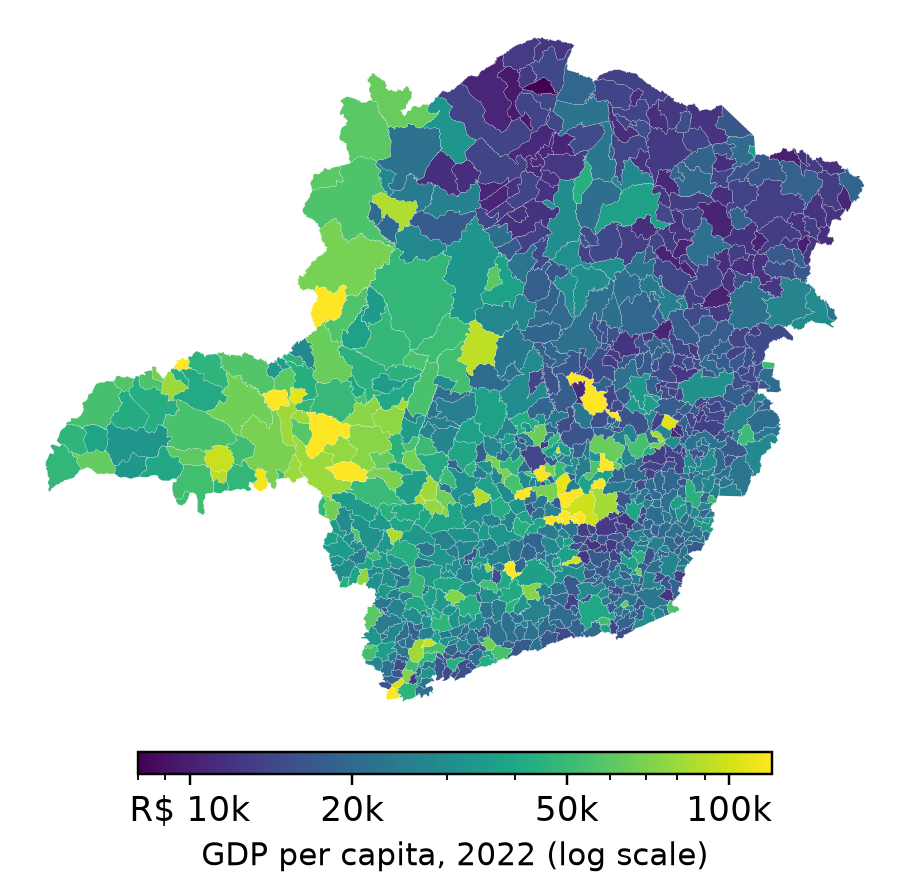
\includegraphics[height=5.5cm]{map_gdp.png}
\column{0.46\textwidth}
{\blackfont\fontsize{34}{36}\selectfont\color{cgdp}\nGdpRatio$\times$}\\[1pt]
{\footnotesize gap in GDP per capita inside one state:\\
\bfseries \nRichName{} \muted{(R\$\,\nRichGdp)} \ vs \ \nPoorName{} \muted{(R\$\,\nPoorGdp)}}\\[8pt]
\begin{itemize}\setlength{\itemsep}{3pt}\footnotesize
  \item Sub-national GDP is published \textbf{late}, \textbf{estimated} from partial data, or \textbf{missing} where statistics are weak.
  \item Satellites measure \textbf{every place, every year, with the same sensor}.
\end{itemize}
\vspace{8pt}
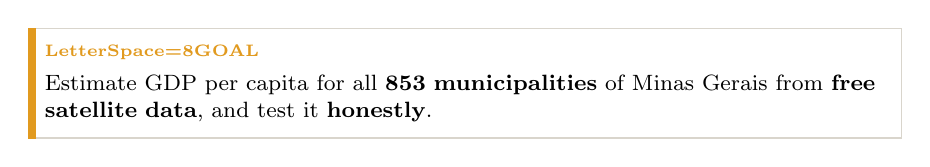
\begin{tikzpicture}
  \node[fill=white,draw=rule,text width=0.88\linewidth,inner sep=6pt,align=left,font=\footnotesize] (g)
    {\eyebrow[cntl]{Goal}\\[3pt]Estimate GDP per capita for all \textbf{\nMunis{} municipalities} of Minas Gerais from
     \textbf{free satellite data}, and test it \textbf{honestly}.};
  \fill[cntl] (g.north west) rectangle ($(g.south west)+(3pt,0)$);
\end{tikzpicture}
\end{columns}
\end{frame}

%======================== 3. TWO IDEAS =================================
\begin{frame}{Two recent ideas, never tested together}
\centering
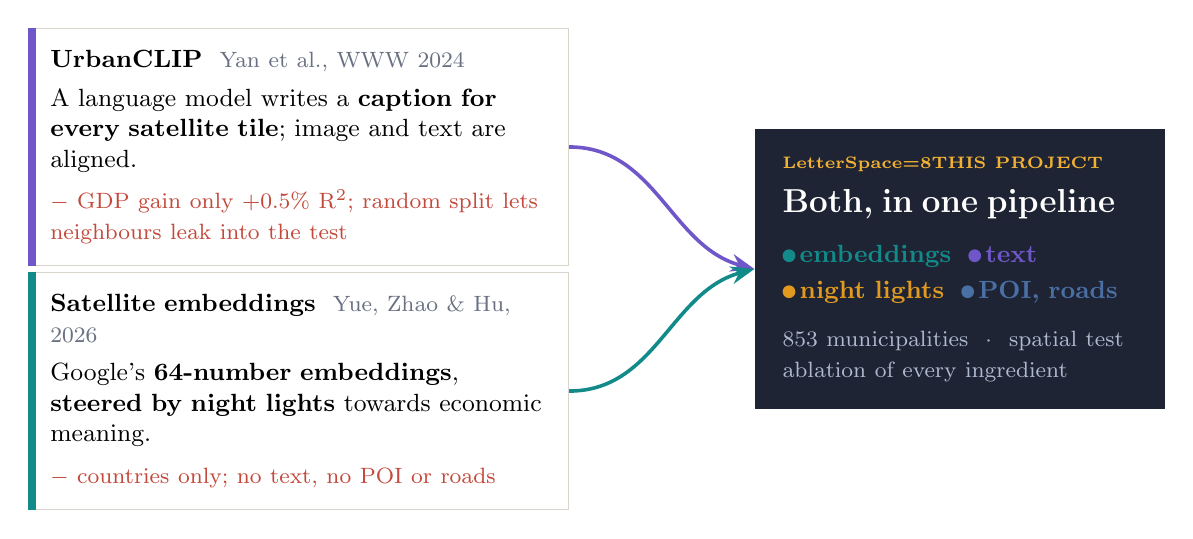
\begin{tikzpicture}[
  card/.style={fill=white,draw=rule,text width=6.3cm,inner sep=8pt,align=left,font=\small},
  arr/.style={-{Stealth[length=3mm]},line width=1.3pt}]
  \node[card] (u) at (0,1.55) {{\bfseries UrbanCLIP} \ \muted{\footnotesize Yan et al., WWW 2024}\\[3pt]
    A language model writes a \textbf{caption for every satellite tile}; image and text are aligned.\\[4pt]
    {\footnotesize\color{cgdp}$-$\ GDP gain only +0.5\% R\textsuperscript{2}; random split lets neighbours leak into the test}};
  \fill[ctxt] (u.north west) rectangle ($(u.south west)+(3pt,0)$);
  \node[card] (e) at (0,-1.55) {{\bfseries Satellite embeddings} \ \muted{\footnotesize Yue, Zhao \& Hu, 2026}\\[3pt]
    Google's \textbf{64-number embeddings}, \textbf{steered by night lights} towards economic meaning.\\[4pt]
    {\footnotesize\color{cgdp}$-$\ countries only; no text, no POI or roads}};
  \fill[cimg] (e.north west) rectangle ($(e.south west)+(3pt,0)$);
  \node[fill=ink,text=white,text width=4.5cm,inner sep=10pt,align=left,font=\small] (o) at (8.4,0)
    {\eyebrow[glow]{This project}\\[5pt]
     {\large\bfseries Both, in one pipeline}\\[7pt]
     \ing{cimg}{embeddings} \ \ing{ctxt}{text}\\[2pt]
     \ing{cntl}{night lights} \ \ing{cpoi}{POI, roads}\\[8pt]
     {\color{haze}\footnotesize \nMunis{} municipalities \ $\cdot$ \ spatial test\\ablation of every ingredient}};
  \draw[arr,ctxt] (u.east) to[out=0,in=165] (o.west);
  \draw[arr,cimg] (e.east) to[out=0,in=195] (o.west);
\end{tikzpicture}
\end{frame}

%======================== 4. PIPELINE ==================================
\setstage{2}
\begin{frame}{Three learning stages, from no labels to official GDP}
\centering
\begin{tikzpicture}[
  thumbcap/.style={font=\fontsize{7}{8.5}\selectfont,align=center,text=ink,inner sep=1pt},
  flow/.style={-{Stealth[length=2.6mm]},line width=1.4pt,draw=ink}]
  \node[stage=ctxt] (A) at (0,0) {\eyebrow[ctxt]{Stage A}\\[2pt]{\bfseries\small Image--text alignment}\\[1pt]embeddings and captions pulled together};
  \node[stage=cntl] (B) at (4.1,0) {\eyebrow[cntl]{Stage B}\\[2pt]{\bfseries\small Night-light steering}\\[1pt]predict each cell's light, keep the inner layer};
  \node[stage=cgdp] (C) at (8.2,0) {\eyebrow[cgdp]{Stage C}\\[2pt]{\bfseries\small Add up the cells}\\[1pt]per municipality, then predict};
  \node[fill=ink,text=white,text width=2.3cm,minimum height=1.6cm,align=center,inner sep=5pt,font=\footnotesize] (Y) at (11.95,0)
    {{\bfseries\small log GDP\\per capita}\\[2pt]{\color{haze}\nMunis{} municipalities}};
  \draw[flow] (A) -- (B); \draw[flow] (B) -- (C); \draw[flow] (C) -- (Y);
  % inputs: the real layers
  \node[inner sep=0] (ti) at (-1.0,2.4) {\framed{cimg}{height=1.2cm}{layer_gsed.png}};
  \node[inner sep=0] (tc) at (1.0,2.4) {\framed{ctxt}{height=1.2cm}{caption_tile.png}};
  \node[inner sep=0] (tn) at (4.1,2.4) {\framed{cntl}{height=1.2cm}{layer_ntl.png}};
  \node[inner sep=0] (tg) at (8.2,2.4) {\framed{cgdp}{height=1.2cm}{layer_gdp.png}};
  \node[thumbcap,above=1pt of ti] {\bfseries embeddings};
  \node[thumbcap,above=1pt of tc] {\bfseries captions + facts};
  \node[thumbcap,above=1pt of tn] {\bfseries night lights};
  \node[thumbcap,above=1pt of tg] {\bfseries official GDP};
  \draw[feed=cimg] (ti.south) -- ($(A.north)+(-1.0,0)$);
  \draw[feed=ctxt] (tc.south) -- ($(A.north)+(1.0,0)$);
  \draw[feed=cntl] (tn) -- (B);
  \draw[feed=cgdp] (tg) -- (C);
  % supervision gets scarcer
  \foreach \n/\t/\c in {A/no labels/ctxt,B/cheap proxy label/cntl,C/853 real labels/cgdp}
    \node[below=4pt of \n,font=\bfseries\fontsize{6.5}{8}\selectfont,text=\c] {\MakeUppercase{\t}};
\end{tikzpicture}
\vspace{4pt}

\fnote{Captions are needed only in training: at prediction time each cell uses its embedding alone.
Switching stages off gives the ablations (variants V3--V9).}
\end{frame}

%======================== 5. DATA ======================================
\setstage{3}
\begin{frame}{Six free layers on one 1\,km grid}
\begin{columns}[c,onlytextwidth]
\column{0.68\textwidth}
\begin{tikzpicture}[
  lname/.style={anchor=west,font=\footnotesize\bfseries,inner sep=0},
  lsrc/.style={anchor=north west,font=\fontsize{6.5}{8}\selectfont,text=muted,inner sep=0,yshift=-2pt}]
  \foreach \img/\c/\name/\src [count=\i from 0] in {
      gsed/cimg/Satellite embeddings/{Google GSED, 64 numbers, 10\,m to 1\,km},
      captions/ctxt/Captioned tiles/{\nCaptions{} Esri tiles, Qwen2.5-VL},
      buildings/ink/Buildings/{Microsoft + OSM footprints},
      roads/cpoi/Roads and POIs/{OpenStreetMap},
      ntl/cntl/Night lights/{VIIRS 2022},
      gdp/cgdp/GDP per capita (target)/{IBGE 2022, official}} {
    \begin{scope}[yshift=\i*0.74cm,cm={1,0.28,-0.62,0.5,(0,0)}]
      \fill[white,draw=\c,line width=0.8pt] (0,0) rectangle (3.0,2.44);
      \node[transform shape,anchor=south west,inner sep=0] at (0,0) {\includegraphics[width=3.0cm,height=2.44cm]{layer_\img.png}};
      \coordinate (r\i) at (3.0,1.22);
    \end{scope}
    \draw[\c,line width=0.5pt] (r\i) -- (r\i -| 4.0,0);
    \fill[\c] (r\i -| 4.0,0) circle (1.5pt);
    \node[lname,text=\c] (n\i) at ($(r\i -| 4.0,0)+(0.15,0.07)$) {\name};
    \node[lsrc] at (n\i.south west) {\src};
  }
\end{tikzpicture}
\column{0.3\textwidth}
\kpi{ink}{\nMunis}{municipalities}\\[6pt]
\kpi{ink}{\nCells}{1\,km cells}\\[6pt]
\kpi{ctxt}{\nCaptions}{captioned tiles}\\[6pt]
\kpi{ink}{\nBuildings}{building footprints}\\[8pt]
\fnote{All layers free and aligned on the same grid (EPSG:31983). The target is official statistics, not night lights.}
\end{columns}
\end{frame}

%======================== 6. CAPTIONS ==================================
\begin{frame}{An AI model describes each tile; map data vetoes false claims}
\begin{columns}[T,onlytextwidth]
\column{0.29\textwidth}
\begin{tikzpicture}
  \node[inner sep=0] (im) {\framed{ctxt}{width=\linewidth}{caption_tile.png}};
  \begin{scope}[x={($(im.south east)-(im.south west)$)},y={($(im.north west)-(im.south west)$)},shift={(im.south west)}]
    \draw[cgdp,line width=1.3pt,dashed] (0.43,0.64) ellipse (0.36 and 0.33);
    \node[anchor=south west,font=\fontsize{6.5}{8}\selectfont\bfseries,fill=white,text=cgdp,inner sep=2pt]
      at (0.03,0.03) {centre-pivot irrigation, not a mine};
  \end{scope}
\end{tikzpicture}\\[2pt]
\fnote{Esri World Imagery, about 1\,m per pixel}
\column{0.38\textwidth}
\eyebrow[ctxt]{Qwen2.5-VL-7B caption, after the checks}\\[-2pt]
\begin{itemize}\setlength{\itemsep}{1pt}\fontsize{7.5}{9}\selectfont
\dropped{The satellite image shows a large circular area with concentric rings, likely a mine pit, surrounded by a grid of smaller rectangular plots of farmland.}{unsupported industry claim}
\keep{Roads crisscross the area, connecting the plots and the perimeter.}
\keep{Vegetation is sparse, mostly along the edges and in some patches within the farmland.}
\keep{A small body of water, possibly a pond, is visible near the farmland.}
\keep{No buildings or industrial structures are evident, suggesting minimal built-up area.}
\dropped{The overall scene appears to be an agricultural landscape with a focus on farming and possibly mining operations.}{filler}

\end{itemize}
\column{0.29\textwidth}
\eyebrow{Sentences removed, by rule}\\[5pt]
\resizebox{\linewidth}{!}{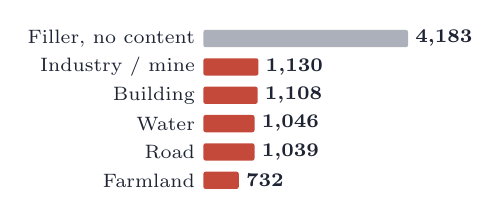
\begin{tikzpicture}[x=1cm,y=1cm,
  lab/.style={font=\fontsize{7.5}{9}\selectfont,text=ink,inner sep=0pt},
  num/.style={font=\bfseries\fontsize{7.5}{9}\selectfont,inner sep=1pt},
  tick/.style={font=\fontsize{6.5}{7.8}\selectfont,text=muted,inner sep=0pt}]
\node[lab,anchor=east] at (-0.1,-0.00) {Filler, no content};
\fill[muted!55,rounded corners=0.8pt] (0,-0.11) rectangle (2.60,0.11);
\node[num,text=ink,anchor=west] at (2.65,-0.00) {4,183};
\node[lab,anchor=east] at (-0.1,-0.36) {Industry / mine};
\fill[cgdp,rounded corners=0.8pt] (0,-0.47) rectangle (0.70,-0.25);
\node[num,text=ink,anchor=west] at (0.75,-0.36) {1,130};
\node[lab,anchor=east] at (-0.1,-0.72) {Building};
\fill[cgdp,rounded corners=0.8pt] (0,-0.83) rectangle (0.69,-0.61);
\node[num,text=ink,anchor=west] at (0.74,-0.72) {1,108};
\node[lab,anchor=east] at (-0.1,-1.08) {Water};
\fill[cgdp,rounded corners=0.8pt] (0,-1.19) rectangle (0.65,-0.97);
\node[num,text=ink,anchor=west] at (0.70,-1.08) {1,046};
\node[lab,anchor=east] at (-0.1,-1.44) {Road};
\fill[cgdp,rounded corners=0.8pt] (0,-1.55) rectangle (0.65,-1.33);
\node[num,text=ink,anchor=west] at (0.70,-1.44) {1,039};
\node[lab,anchor=east] at (-0.1,-1.80) {Farmland};
\fill[cgdp,rounded corners=0.8pt] (0,-1.91) rectangle (0.45,-1.69);
\node[num,text=ink,anchor=west] at (0.50,-1.80) {732};
\end{tikzpicture}
}\\[8pt]
{\blackfont\fontsize{20}{22}\selectfont\color{okc}\nKept}\ {\footnotesize kept of \nSentences{} sentences}\\[3pt]
\fnote{Checked against ESA land cover, OSM roads and building footprints; image--text matching removes \nClipDropped{} more captions.
A blind hand audit is in progress.}
\end{columns}
\end{frame}

%======================== 7. TEST ======================================
\setstage{4}
\begin{frame}{Every municipality is tested in a region never seen}
\begin{columns}[c,onlytextwidth]
\column{0.47\textwidth}
\centering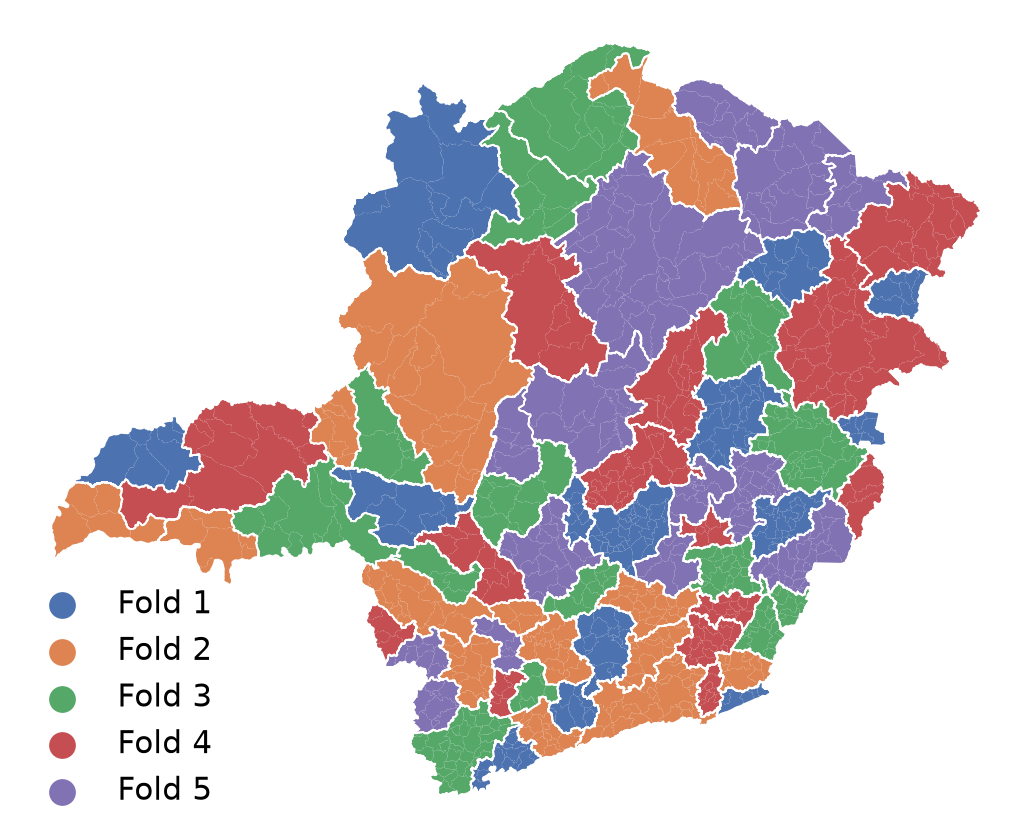
\includegraphics[height=5.3cm]{map_folds.png}\\[-2pt]
\fnote{70 official regions (white outlines) grouped into 5 folds}
\column{0.5\textwidth}
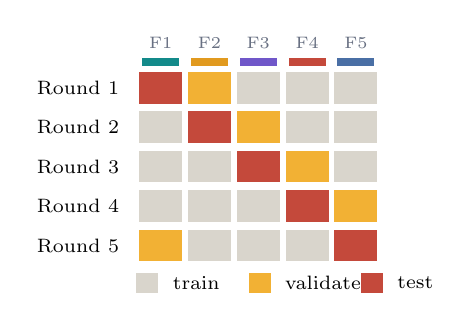
\begin{tikzpicture}[x=0.62cm,y=0.5cm]
  \foreach \c [count=\f from 0] in {cimg,cntl,ctxt,cgdp,cpoi} {
    \fill[\c] (\f+0.12,0.55) rectangle (\f+0.88,0.75);
    \node[font=\fontsize{6.5}{8}\selectfont,text=muted] at (\f+0.5,1.15) {F\the\numexpr\f+1\relax};
  }
  \foreach \r in {0,...,4} {
    \node[anchor=east,font=\fontsize{7}{8}\selectfont] at (-0.15,-\r) {Round \the\numexpr\r+1\relax};
    \pgfmathtruncatemacro\v{mod(\r+1,5)}
    \foreach \f in {0,...,4} {
      \ifnum\f=\r \def\fc{cgdp}\else\ifnum\f=\v \def\fc{glow}\else\def\fc{rule}\fi\fi
      \fill[\fc] (\f+0.06,-\r-0.4) rectangle (\f+0.94,-\r+0.4);
    }
  }
  \foreach \c/\t [count=\k from 0] in {rule/train,glow/validate,cgdp/test} {
    \fill[\c] (\k*2.3,-5.2) rectangle ++(0.45,0.5);
    \node[anchor=west,font=\fontsize{7}{8}\selectfont] at (\k*2.3+0.55,-4.95) {\t};
  }
\end{tikzpicture}\\[8pt]
\begin{itemize}\setlength{\itemsep}{3pt}\footnotesize
  \item Whole regions held out: \textbf{no look-alike neighbour} in training. All stages retrained each round.
  \item UrbanCLIP split tiles \textbf{at random}, so neighbours sat on both sides and scores were inflated.
\end{itemize}
\vspace{2pt}
\fnote{Models are compared on the same folds with a block bootstrap over regions (95\% intervals).}
\end{columns}
\end{frame}

%======================== 8. RESULTS ===================================
\setstage{5}
\begin{frame}{Text gives the biggest gain; the hybrid explains half of GDP}
\begin{columns}[c,onlytextwidth]
\column{0.62\textwidth}
\resizebox{!}{5.2cm}{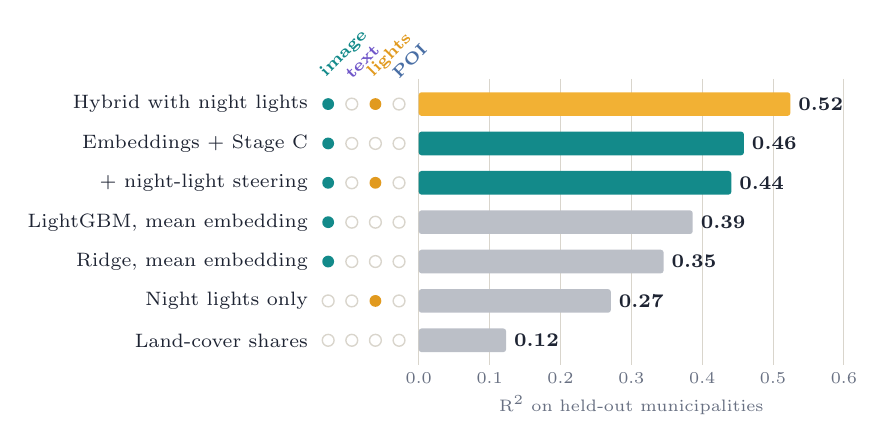
\begin{tikzpicture}[x=1cm,y=1cm,
  lab/.style={font=\fontsize{7.5}{9}\selectfont,text=ink,inner sep=0pt},
  num/.style={font=\bfseries\fontsize{7.5}{9}\selectfont,inner sep=1pt},
  tick/.style={font=\fontsize{6.5}{7.8}\selectfont,text=muted,inner sep=0pt}]
\node[tick,text=cimg,font=\bfseries\fontsize{6}{7}\selectfont,rotate=45,anchor=south west] at (-1.15,0.3) {image};
\node[tick,text=ctxt,font=\bfseries\fontsize{6}{7}\selectfont,rotate=45,anchor=south west] at (-0.85,0.3) {text};
\node[tick,text=cntl,font=\bfseries\fontsize{6}{7}\selectfont,rotate=45,anchor=south west] at (-0.55,0.3) {lights};
\node[tick,text=cpoi,font=\bfseries\fontsize{6}{7}\selectfont,rotate=45,anchor=south west] at (-0.25,0.3) {POI};
\draw[rule,line width=0.4pt] (0.00,0.32) -- (0.00,-3.32);
\node[tick,anchor=north] at (0.00,-3.40) {0.0};
\draw[rule,line width=0.4pt] (0.90,0.32) -- (0.90,-3.32);
\node[tick,anchor=north] at (0.90,-3.40) {0.1};
\draw[rule,line width=0.4pt] (1.80,0.32) -- (1.80,-3.32);
\node[tick,anchor=north] at (1.80,-3.40) {0.2};
\draw[rule,line width=0.4pt] (2.70,0.32) -- (2.70,-3.32);
\node[tick,anchor=north] at (2.70,-3.40) {0.3};
\draw[rule,line width=0.4pt] (3.60,0.32) -- (3.60,-3.32);
\node[tick,anchor=north] at (3.60,-3.40) {0.4};
\draw[rule,line width=0.4pt] (4.50,0.32) -- (4.50,-3.32);
\node[tick,anchor=north] at (4.50,-3.40) {0.5};
\draw[rule,line width=0.4pt] (5.40,0.32) -- (5.40,-3.32);
\node[tick,anchor=north] at (5.40,-3.40) {0.6};
\node[tick,anchor=north] at (2.70,-3.70) {R\textsuperscript{2} on held-out municipalities};
\node[lab,anchor=east] at (-1.4,-0.00) {Hybrid with night lights};
\path[fill=cimg] (-1.15,-0.00) circle (0.075);
\path[draw=rule,line width=0.5pt,fill=white] (-0.85,-0.00) circle (0.075);
\path[fill=cntl] (-0.55,-0.00) circle (0.075);
\path[draw=rule,line width=0.5pt,fill=white] (-0.25,-0.00) circle (0.075);
\fill[glow,rounded corners=1pt] (0,-0.15) rectangle (4.72,0.15);
\node[num,anchor=west,text=ink] at (4.78,-0.00) {0.52};
\node[lab,anchor=east] at (-1.4,-0.50) {Embeddings + Stage C};
\path[fill=cimg] (-1.15,-0.50) circle (0.075);
\path[draw=rule,line width=0.5pt,fill=white] (-0.85,-0.50) circle (0.075);
\path[draw=rule,line width=0.5pt,fill=white] (-0.55,-0.50) circle (0.075);
\path[draw=rule,line width=0.5pt,fill=white] (-0.25,-0.50) circle (0.075);
\fill[cimg,rounded corners=1pt] (0,-0.65) rectangle (4.13,-0.35);
\node[num,anchor=west,text=ink] at (4.19,-0.50) {0.46};
\node[lab,anchor=east] at (-1.4,-1.00) {+ night-light steering};
\path[fill=cimg] (-1.15,-1.00) circle (0.075);
\path[draw=rule,line width=0.5pt,fill=white] (-0.85,-1.00) circle (0.075);
\path[fill=cntl] (-0.55,-1.00) circle (0.075);
\path[draw=rule,line width=0.5pt,fill=white] (-0.25,-1.00) circle (0.075);
\fill[cimg,rounded corners=1pt] (0,-1.15) rectangle (3.97,-0.85);
\node[num,anchor=west,text=ink] at (4.03,-1.00) {0.44};
\node[lab,anchor=east] at (-1.4,-1.50) {LightGBM, mean embedding};
\path[fill=cimg] (-1.15,-1.50) circle (0.075);
\path[draw=rule,line width=0.5pt,fill=white] (-0.85,-1.50) circle (0.075);
\path[draw=rule,line width=0.5pt,fill=white] (-0.55,-1.50) circle (0.075);
\path[draw=rule,line width=0.5pt,fill=white] (-0.25,-1.50) circle (0.075);
\fill[muted!45,rounded corners=1pt] (0,-1.65) rectangle (3.48,-1.35);
\node[num,anchor=west,text=ink] at (3.54,-1.50) {0.39};
\node[lab,anchor=east] at (-1.4,-2.00) {Ridge, mean embedding};
\path[fill=cimg] (-1.15,-2.00) circle (0.075);
\path[draw=rule,line width=0.5pt,fill=white] (-0.85,-2.00) circle (0.075);
\path[draw=rule,line width=0.5pt,fill=white] (-0.55,-2.00) circle (0.075);
\path[draw=rule,line width=0.5pt,fill=white] (-0.25,-2.00) circle (0.075);
\fill[muted!45,rounded corners=1pt] (0,-2.15) rectangle (3.11,-1.85);
\node[num,anchor=west,text=ink] at (3.17,-2.00) {0.35};
\node[lab,anchor=east] at (-1.4,-2.50) {Night lights only};
\path[draw=rule,line width=0.5pt,fill=white] (-1.15,-2.50) circle (0.075);
\path[draw=rule,line width=0.5pt,fill=white] (-0.85,-2.50) circle (0.075);
\path[fill=cntl] (-0.55,-2.50) circle (0.075);
\path[draw=rule,line width=0.5pt,fill=white] (-0.25,-2.50) circle (0.075);
\fill[muted!45,rounded corners=1pt] (0,-2.65) rectangle (2.44,-2.35);
\node[num,anchor=west,text=ink] at (2.50,-2.50) {0.27};
\node[lab,anchor=east] at (-1.4,-3.00) {Land-cover shares};
\path[draw=rule,line width=0.5pt,fill=white] (-1.15,-3.00) circle (0.075);
\path[draw=rule,line width=0.5pt,fill=white] (-0.85,-3.00) circle (0.075);
\path[draw=rule,line width=0.5pt,fill=white] (-0.55,-3.00) circle (0.075);
\path[draw=rule,line width=0.5pt,fill=white] (-0.25,-3.00) circle (0.075);
\fill[muted!45,rounded corners=1pt] (0,-3.15) rectangle (1.11,-2.85);
\node[num,anchor=west,text=ink] at (1.17,-3.00) {0.12};
\end{tikzpicture}
}\\[2pt]
\fnote{Dots: ingredients each model uses. Hybrid = best model blended with night lights.}
\column{0.34\textwidth}
{\blackfont\fontsize{24}{26}\selectfont\color{ink}\nHybridR}\ \ {\fontsize{7.5}{9}\selectfont\color{muted}R\textsuperscript{2}, hybrid, unseen regions}\\[8pt]
\chip{ctxt}{RQ2 \ TEXT} \ {\footnotesize\bfseries largest gain, borderline}\\[-1pt]\fnote{\RQtwo}\\[5pt]
\chip{muted}{RQ1 \ STEERING} \ {\footnotesize\bfseries no clear effect}\\[-1pt]\fnote{\RQone}\\[5pt]
\chip{muted}{RQ3 \ POI, ROADS} \ {\footnotesize\bfseries nothing added}\\[-1pt]\fnote{\RQthree}\\[5pt]
\chip{cntl}{RQ4 \ HYBRID} \ {\footnotesize\bfseries best, not significant}\\[-1pt]\fnote{\RQfour}\\[5pt]
\fnote{RMSE differences on log GDP per capita with 95\% block-bootstrap intervals; negative = first model better.}
\end{columns}
\end{frame}

%======================== 9. MAPS ======================================
\begin{frame}{Predictions follow the map, but are pulled towards the middle}
\begin{columns}[T,onlytextwidth]
\column{0.28\textwidth}\centering
\eyebrow[cgdp]{Official}\\[2pt]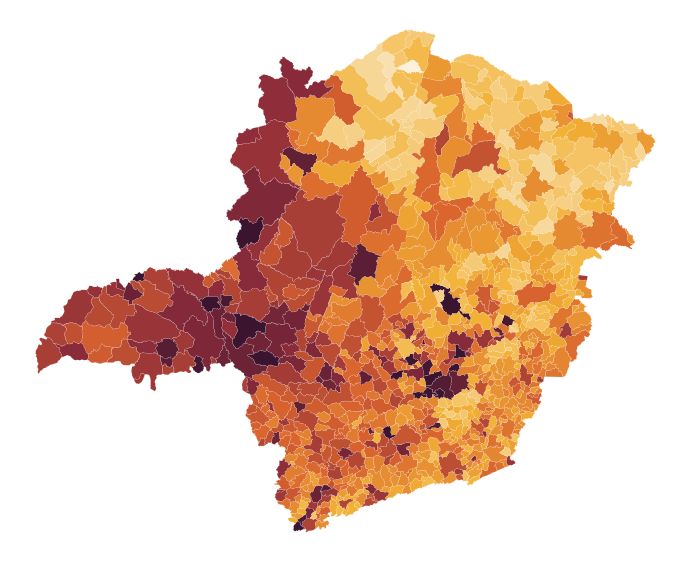
\includegraphics[width=\linewidth]{map_official.png}
\column{0.28\textwidth}\centering
\eyebrow[cgdp]{Predicted (hybrid)}\\[2pt]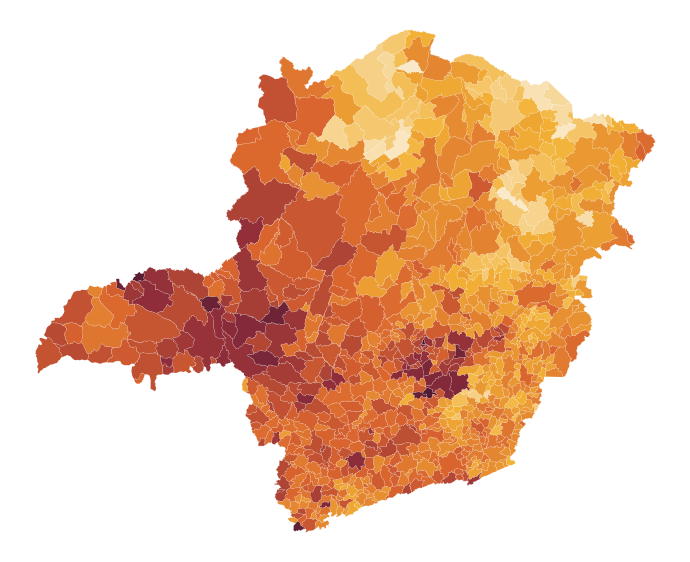
\includegraphics[width=\linewidth]{map_predicted.png}
\column{0.28\textwidth}\centering
\eyebrow{Error}\\[2pt]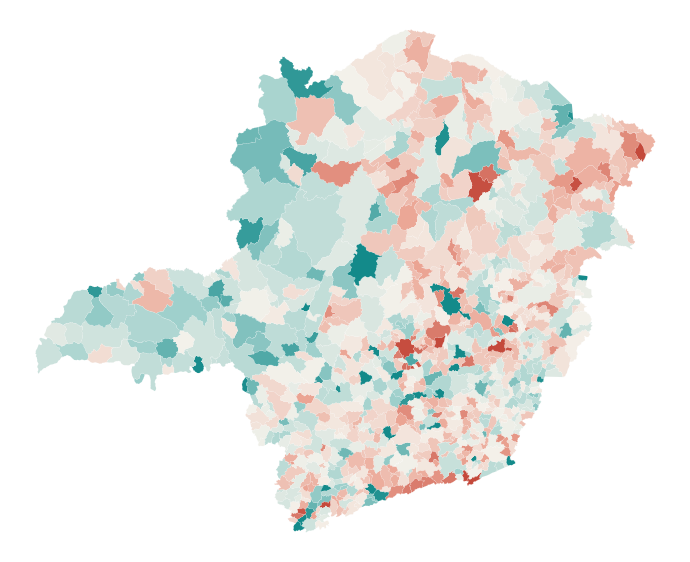
\includegraphics[width=\linewidth]{map_error.png}
\column{0.12\textwidth}
\end{columns}
\begin{columns}[T,onlytextwidth]
\column{0.56\textwidth}\centering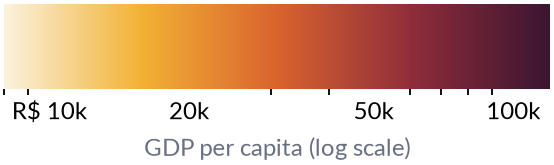
\includegraphics[width=0.5\linewidth]{cbar_gdp.png}
\column{0.28\textwidth}\centering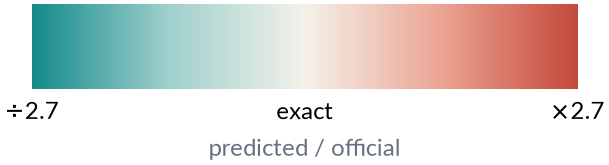
\includegraphics[width=0.85\linewidth]{cbar_err.png}
\column{0.12\textwidth}
\end{columns}
\vspace{8pt}
\begin{columns}[T,onlytextwidth]
\column{0.24\textwidth}
{\blackfont\fontsize{20}{22}\selectfont\color{ink}\nWithinHalf}\\{\fontsize{7}{8.5}\selectfont\color{muted}of municipalities predicted within a factor 1.5 of official}
\column{0.74\textwidth}
\footnotesize \textcolor{cimg}{\textbf{Under-predicted:}} rich agribusiness and mining towns (west, centre).\\[2pt]
\textcolor{cgdp}{\textbf{Over-predicted:}} the poorer north-east. \ \muted{Explaining these errors is RQ5, next.}
\end{columns}
\end{frame}

%======================== 10. LESSONS ==================================
\begin{frame}{Calibration mattered more than night-light steering}
\begin{columns}[c,onlytextwidth]
\column{0.46\textwidth}
\centering\resizebox{\linewidth}{!}{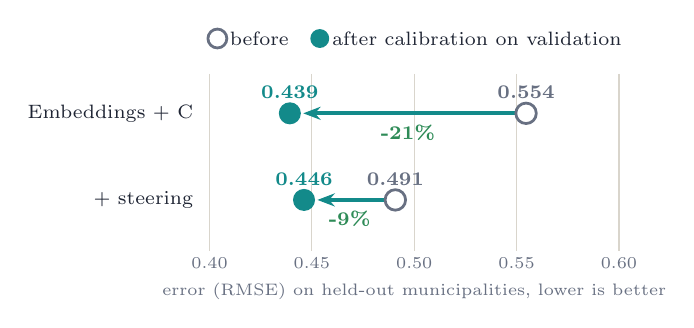
\begin{tikzpicture}[x=1cm,y=1cm,
  lab/.style={font=\fontsize{7.5}{9}\selectfont,text=ink,inner sep=0pt},
  num/.style={font=\bfseries\fontsize{7.5}{9}\selectfont,inner sep=1pt},
  tick/.style={font=\fontsize{6.5}{7.8}\selectfont,text=muted,inner sep=0pt}]
\draw[rule,line width=0.4pt] (0.00,0.5) -- (0.00,-1.75);
\node[tick,anchor=north] at (0.00,-1.83) {0.40};
\draw[rule,line width=0.4pt] (1.30,0.5) -- (1.30,-1.75);
\node[tick,anchor=north] at (1.30,-1.83) {0.45};
\draw[rule,line width=0.4pt] (2.60,0.5) -- (2.60,-1.75);
\node[tick,anchor=north] at (2.60,-1.83) {0.50};
\draw[rule,line width=0.4pt] (3.90,0.5) -- (3.90,-1.75);
\node[tick,anchor=north] at (3.90,-1.83) {0.55};
\draw[rule,line width=0.4pt] (5.20,0.5) -- (5.20,-1.75);
\node[tick,anchor=north] at (5.20,-1.83) {0.60};
\node[tick,anchor=north] at (2.60,-2.15) {error (RMSE) on held-out municipalities, lower is better};
\node[lab,anchor=east] at (-0.2,-0.00) {Embeddings + C};
\draw[-{Stealth[length=2.2mm]},cimg,line width=1.4pt] (3.88,-0.00) -- (1.19,-0.00);
\node[circle,draw=muted,fill=white,line width=1pt,minimum size=2.6mm,inner sep=0pt] at (4.02,-0.00) {};
\node[circle,fill=cimg,minimum size=2.8mm,inner sep=0pt] at (1.02,-0.00) {};
\node[num,text=muted,anchor=south] at (4.02,0.14) {0.554};
\node[num,text=cimg,anchor=south] at (1.02,0.14) {0.439};
\node[num,text=okc,anchor=north] at (2.52,-0.10) {-21\%};
\node[lab,anchor=east] at (-0.2,-1.10) {+ steering};
\draw[-{Stealth[length=2.2mm]},cimg,line width=1.4pt] (2.22,-1.10) -- (1.37,-1.10);
\node[circle,draw=muted,fill=white,line width=1pt,minimum size=2.6mm,inner sep=0pt] at (2.36,-1.10) {};
\node[circle,fill=cimg,minimum size=2.8mm,inner sep=0pt] at (1.20,-1.10) {};
\node[num,text=muted,anchor=south] at (2.36,-0.96) {0.491};
\node[num,text=cimg,anchor=south] at (1.20,-0.96) {0.446};
\node[num,text=okc,anchor=north] at (1.78,-1.20) {-9\%};
\node[circle,draw=muted,fill=white,line width=1pt,minimum size=2.4mm,inner sep=0pt] at (0.1,0.95) {};
\node[lab,anchor=west] at (0.25,0.95) {before};
\node[circle,fill=cimg,minimum size=2.4mm,inner sep=0pt] at (1.4,0.95) {};
\node[lab,anchor=west] at (1.55,0.95) {after calibration on validation};
\end{tikzpicture}
}
\column{0.5\textwidth}
\begin{enumerate}\setlength{\itemsep}{9pt}\small
  \item \textbf{Predictions were over-spread.} A straight-line correction fitted on validation municipalities
        cut error by {\bfseries\color{okc}\nCalibGain}.
  \item \textbf{Honest testing changes conclusions.} Steering looked helpful before the fix; after it, the gain vanished.
  \item \textbf{Captions need checking.} The model invents mines, roads and farmland on plain tiles;
        the data checks remove most of it.
\end{enumerate}
\end{columns}
\end{frame}

%======================== 11. PROGRESS =================================
\setstage{6}
\begin{frame}{Status}
\begin{columns}[T,onlytextwidth]
\column{0.55\textwidth}
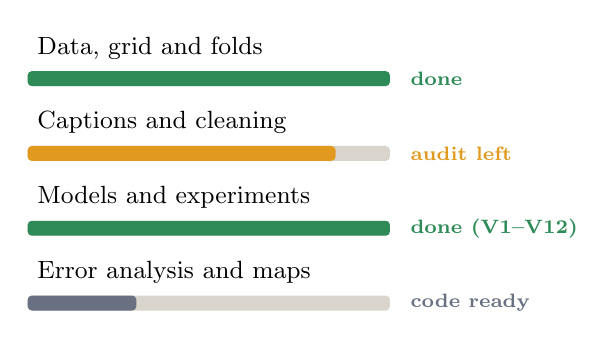
\begin{tikzpicture}[x=4.6cm,y=0.95cm]
  \foreach \lab/\pct/\fc/\st [count=\i] in {
      {Data, grid and folds}/1.00/okc/done,
      {Captions and cleaning}/0.85/cntl/audit left,
      {Models and experiments}/1.00/okc/done (V1--V12),
      {Error analysis and maps}/0.30/muted/code ready} {
    \node[anchor=west,font=\small] at (0,-\i+0.24) {\lab};
    \fill[rule,rounded corners=1.5pt] (0,-\i-0.07) rectangle (1,-\i-0.27);
    \fill[\fc,rounded corners=1.5pt] (0,-\i-0.07) rectangle (\pct,-\i-0.27);
    \node[anchor=west,font=\bfseries\fontsize{7}{8}\selectfont,text=\fc] at (1.03,-\i-0.17) {\st};
  }
\end{tikzpicture}
\column{0.41\textwidth}
\eyebrow{Research questions}\\[4pt]
{\renewcommand{\arraystretch}{1.3}\small
\begin{tabular}{@{}L{3.6cm}l@{}}
RQ1 \ night-light steering & \chip{okc}{ANSWERED}\\
RQ2 \ text (captions) & \chip{okc}{ANSWERED}\\
RQ3 \ POIs and roads & \chip{okc}{ANSWERED}\\
RQ4 \ hybrid & \chip{okc}{ANSWERED}\\
RQ5 \ where it fails & \chip{muted}{NEXT}\\
\end{tabular}}\\[10pt]
\eyebrow{Next}\\[3pt]
{\small caption audit \ $\rightarrow$ \ error analysis and 1\,km maps (RQ5) \ $\rightarrow$ \ report}
\end{columns}
\end{frame}

%======================== 12. CLOSING (night) ==========================
{\setbeamertemplate{background}{\nightbg}
\begin{frame}[plain]
\begin{tikzpicture}[remember picture,overlay]
  \node[anchor=east,inner sep=0,opacity=0.55] at ($(current page.east)+(0.3,0)$)
    {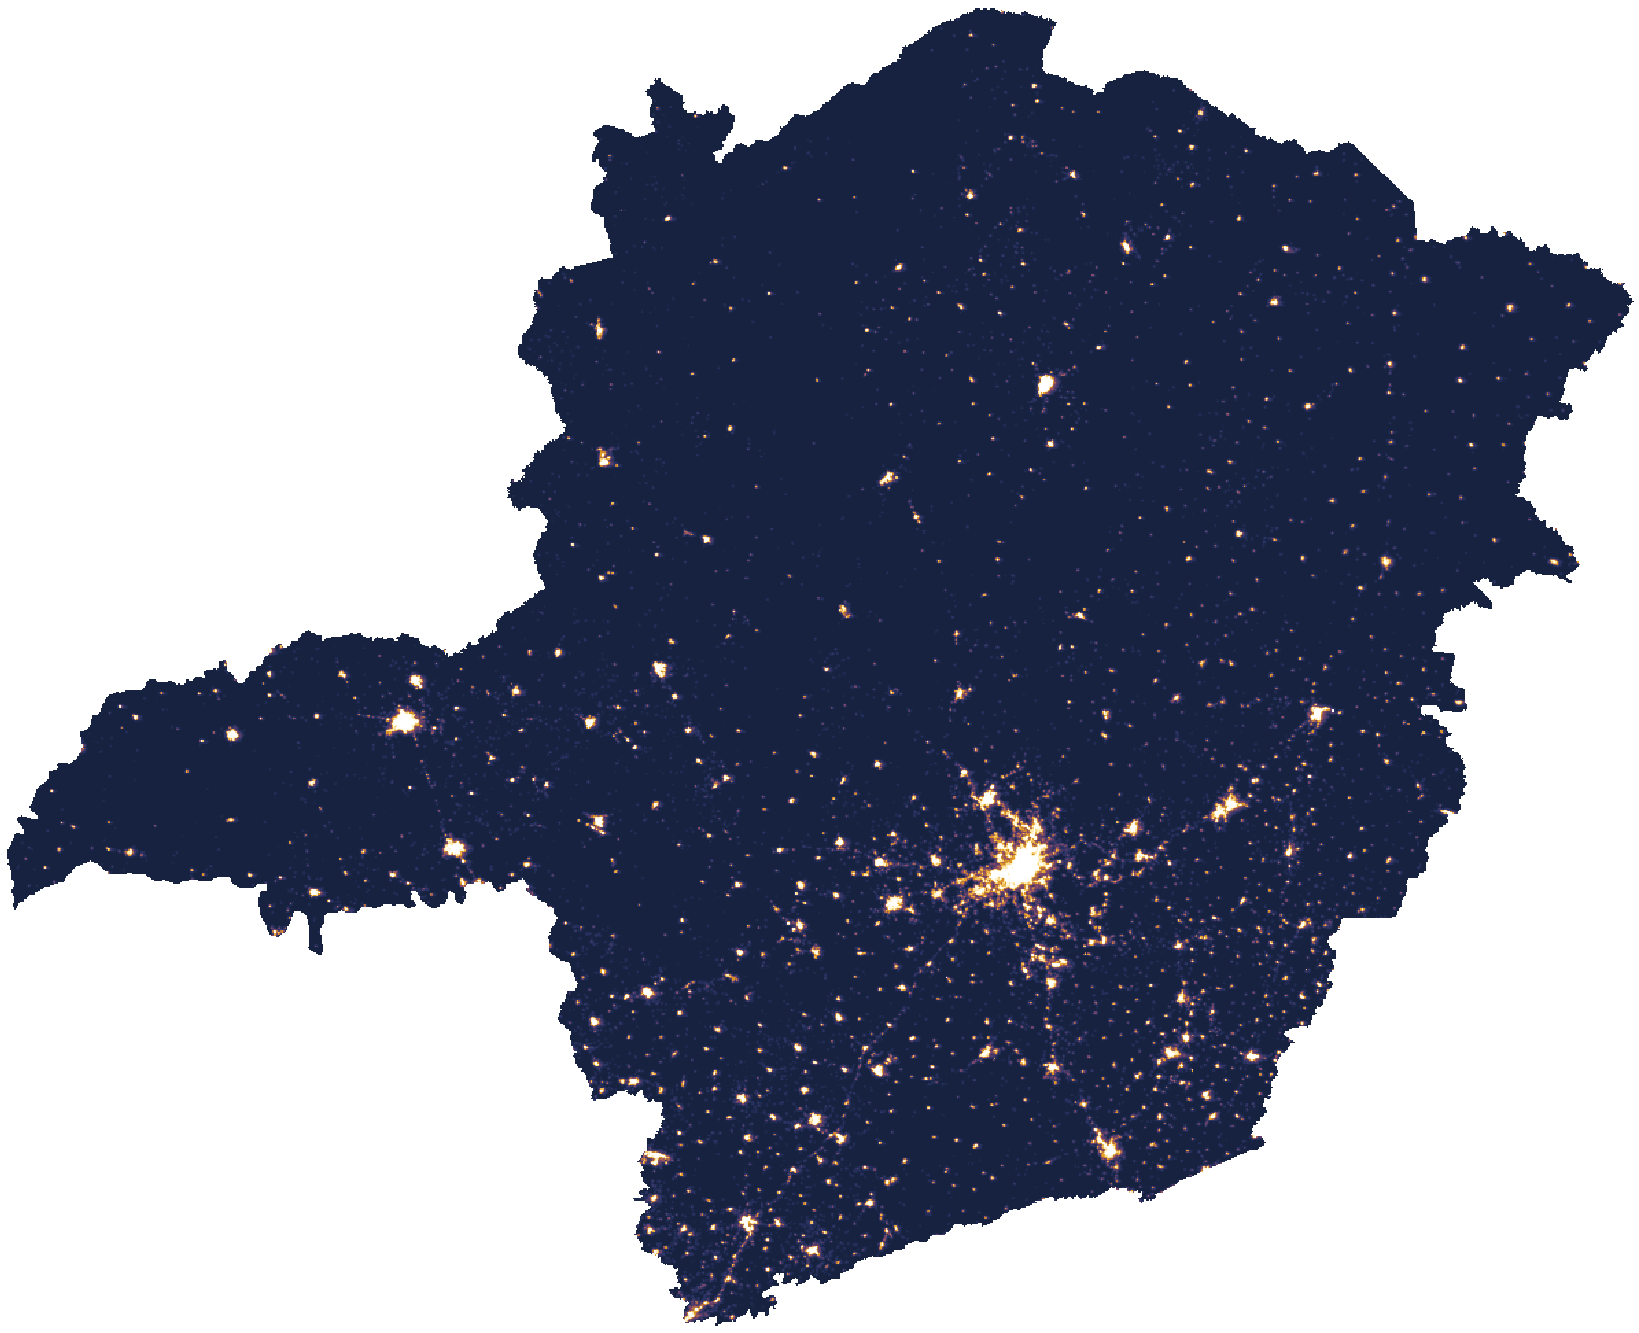
\includegraphics[height=0.9\paperheight]{hero_ntl.png}};
\end{tikzpicture}
\begin{minipage}{0.64\textwidth}\raggedright
\eyebrow[glow]{So far}\\[8pt]
{\blackfont\fontsize{17}{21}\selectfont\color{white}Satellite embeddings, captions and night lights, tested honestly, explain half of local GDP.\par}
\vspace{14pt}
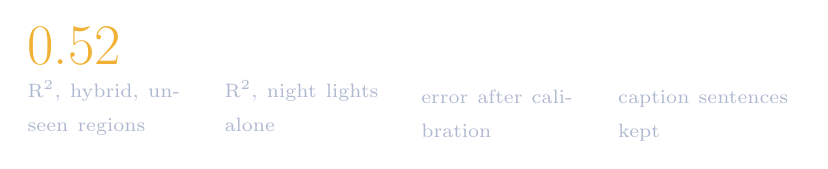
\begin{tikzpicture}[k/.style={anchor=north west,text width=2.3cm,align=left,inner sep=0}]
  \node[k] at (0,0) {{\blackfont\fontsize{22}{24}\selectfont\color{glow}\nHybridR}\\{\fontsize{7}{8.5}\selectfont\color{haze}R\textsuperscript{2}, hybrid, unseen regions}};
  \node[k] at (2.5,0) {{\blackfont\fontsize{22}{24}\selectfont\color{white}\nNtlR}\\{\fontsize{7}{8.5}\selectfont\color{haze}R\textsuperscript{2}, night lights alone}};
  \node[k] at (5.0,0) {{\blackfont\fontsize{22}{24}\selectfont\color{white}\nCalibGain}\\{\fontsize{7}{8.5}\selectfont\color{haze}error after calibration}};
  \node[k] at (7.5,0) {{\blackfont\fontsize{22}{24}\selectfont\color{white}\nKept}\\{\fontsize{7}{8.5}\selectfont\color{haze}caption sentences kept}};
\end{tikzpicture}
\vspace{14pt}

{\footnotesize\color{haze}\textbf{\color{white}So far:} captions give the largest gain, POIs and steering add nothing clear.
\textbf{\color{white}Next:} where does the model fail (RQ5)?}\\[16pt]
{\blackfont\fontsize{16}{18}\selectfont\color{white}Questions?}\\[3pt]
{\fontsize{7.5}{9}\selectfont\color{haze}github.com/chadsaras/GIS\_Project}
\end{minipage}
\end{frame}}

\end{document}
